\epigraph{Die Schwäche der Gravitation ist keine Schwäche --- sie ist eine geometrische Verdünnung.}{}

\section{G ist abgeleitet, nicht fundamental}


\begin{figure}[htbp]
\centering
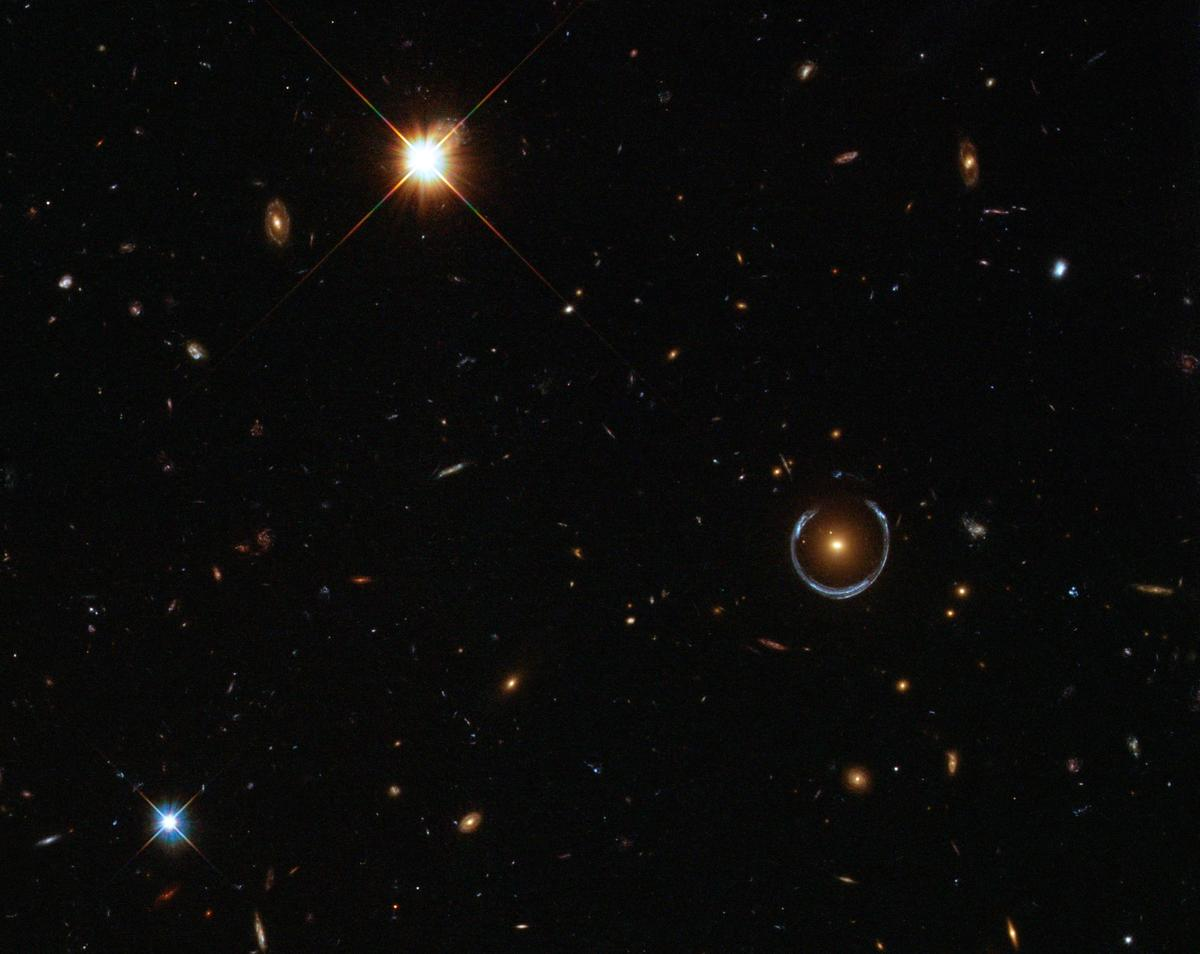
\includegraphics[width=0.85\textwidth]{img/einstein_ring_big.jpg}
\caption{Ein Einstein-Ring (Hubble): Gravitationslinseneffekt. In T0 ist Lichtablenkung kohärente Phasenkrümmung des Vakuumfeldes. Credit: NASA/ESA Hubble.}
\end{figure}
Newton hat die Gravitationskonstante~$G$ eingeführt, um seine Gleichung $F = G m_1 m_2 / r^2$ dimensionsmäßig konsistent zu machen. Seitdem wird $G$ als fundamentale Konstante der Natur behandelt --- eine Zahl, die man messen muss und die keiner tieferen Erklärung zugänglich ist.

In der T0-Theorie ist das anders. $G$ ist kein unabhängiger Parameter. Er folgt aus~$\xsi$:
\begin{equation}
G = \frac{\xsi^2}{4\,m_e} \times C_{\text{conv}} \times \Kfrak
\end{equation}

Das ist keine Anpassung. Es ist eine \emph{Ableitung}. $G$ ergibt sich mit dem experimentell gemessenen Wert $G_{\text{SI}} = 6{,}67 \times 10^{-11}\;\text{m}^3/(\text{kg}\cdot\text{s}^2)$ --- rekonstruierbar allein aus~$\xsi$.

\section{Warum die Gravitation so schwach ist}

Die \enquote{Schwäche} der Gravitation --- die Tatsache, dass sie um rund~$10^{39}$ Größenordnungen schwächer ist als die elektromagnetische Kraft --- gehört zu den großen ungelösten Rätseln der Physik. Es ist das berühmte \emph{Hierarchieproblem}: Warum ist die Gravitation so unglaublich schwach im Vergleich zu allen anderen Kräften?

Die Antwort in T0 ist überraschend einfach: $G$ geht wie~$\xsi^2$. Da $\xsi \approx 1{,}33 \times 10^{-4}$, ist $\xsi^2 \approx 1{,}78 \times 10^{-8}$. Die scheinbare Schwäche der Gravitation ist nichts anderes als die Tatsache, dass $\xsi$ klein ist --- und $\xsi$ ist klein, weil die Raumzeit fast perfekt dreidimensional ist ($\Df = 3 - \xsi \approx 2{,}9999$).

Es gibt kein Hierarchieproblem. Es gibt nur eine geometrische Verdünnung.

\section{Die Planck-Länge als geometrische Größe}

Aus $G$ folgt die Planck-Länge. In natürlichen Einheiten ($c = \hbar = 1$):
\begin{equation}
\lP = \sqrt{G} = \frac{\xsi}{2\sqrt{m_e}}
\end{equation}

(In SI-Einheiten wird $\lP = \sqrt{\hbar G/c^3} \approx 1{,}616 \times 10^{-35}$~m.)

Das ist bemerkenswert. Die Planck-Länge --- traditionell die \enquote{kleinste sinnvolle Länge} der Physik, an der die Quantengravitation relevant wird --- ist in T0 eine rein geometrische Konsequenz von~$\xsi$ und der Elektronmasse.

Und hier schließt sich ein Kreis: Die Planck-Länge, berechnet aus dem experimentell gemessenen~$G$, stimmt \emph{exakt} überein mit der Planck-Länge, berechnet aus~$\xsi$. Warum? Weil beide Berechnungen dieselbe geometrische Realität beschreiben --- nur aus verschiedenen Blickwinkeln.

\begin{kerngedanke}
Die tiefere Erkenntnis: $G$ kodiert die Kopplung zwischen der $\xsi$-Geometrie und der Materie. Die Gravitationskonstante \enquote{misst} nicht die Stärke einer Kraft --- sie beschreibt, wie die Torsion der Raumzeit auf Masseverteilungen reagiert.
\end{kerngedanke}
